\section{Otros Videojuegos que fomentan el PC}
De cara al desarrollo de EcoRescue, se hizo una investigación preliminar para buscar referencias en lo referente al PC en la industria del videojuego. Esta investigación desveló desde un primer momento que los primeros juegos que pueden venir a la mente cuando se habla de PC suelen ser videojuegos muy densos intrínsecamente relacionados con la programación o la algoritmia. Sin ir más lejos, TIS-100\cite{TIS-100} (Figura \ref{fig:tis100}) es uno de los primeros ejemplos que se pueden encontrar si se buscan juegos del estilo, y es nada más y nada menos que un videojuego sobre programar en ensamblador. 

\begin{figure}[H]
    \centering
      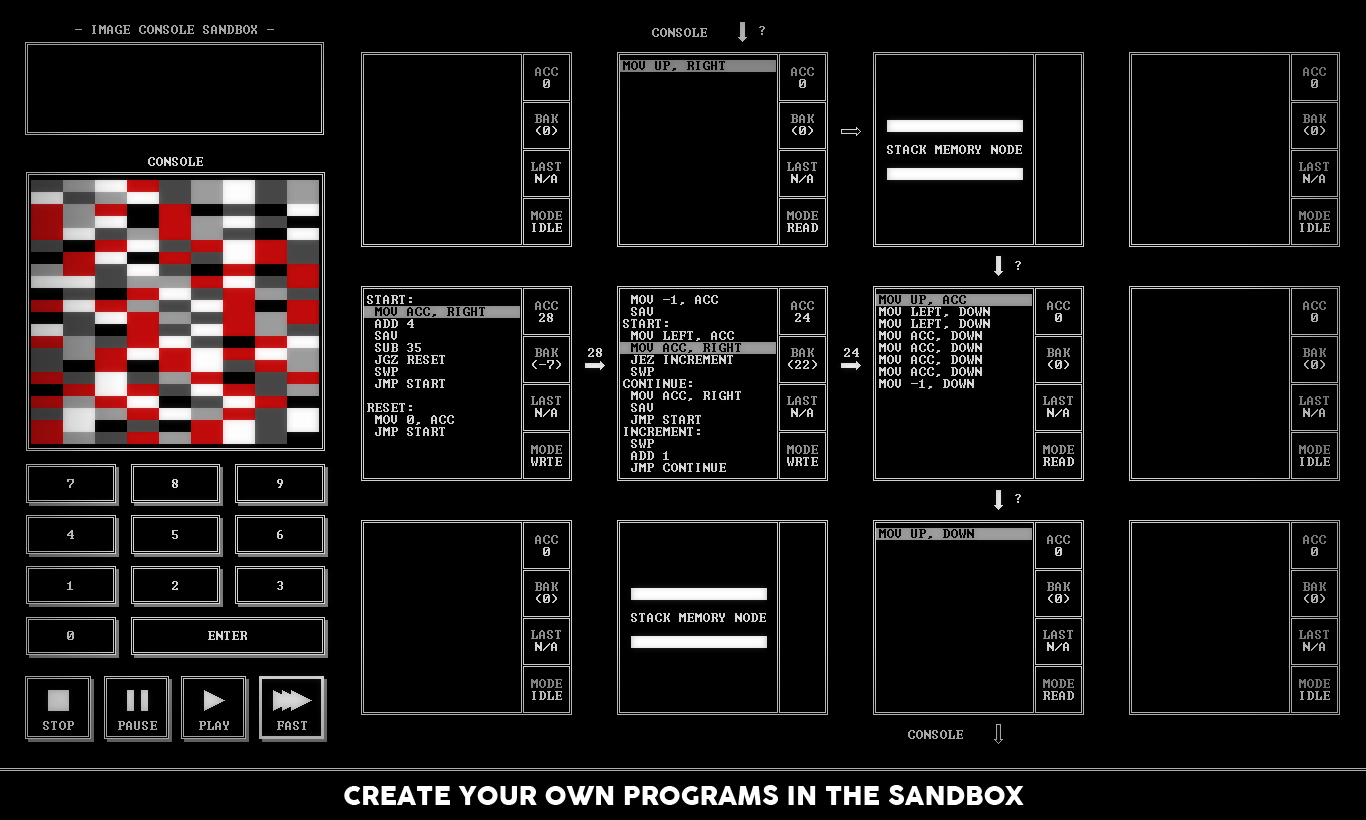
\includegraphics[width=350px,clip=true]{TIS.jpg}
    \caption{TIS-100}
    \label{fig:tis100}
\end{figure}

Sin necesidad de ir a ejemplos tan extremos, la mayoría de juegos reconocidos por ayudar a desarrollar en mayor o menor medida el PC suelen ser juegos con mecánicas muy similares a TIS-100, dado que estas permiten entrenar la mayoría de aspectos del PC Generalización, Algoritmia, Análisis de Datos, Depuración de Errores..., podemos encontrar un gameplay similar en juegos del mismo creador como SpaceChem\cite{SpaceChem} (Figura \ref{fig:spaceChem}), o juegos de otros desarrolladores, como lo pueden ser Human Resource Machine\cite{hrsm} (Figura \ref{fig:hsrm}) o LightBot\cite{lightbot} (Figura \ref{fig:lightbot}), dos juegos muy similares cuyo gameplay es muy similar a programar en Scratch\cite{Scratch}.

\begin{figure}[H]
    \centering
      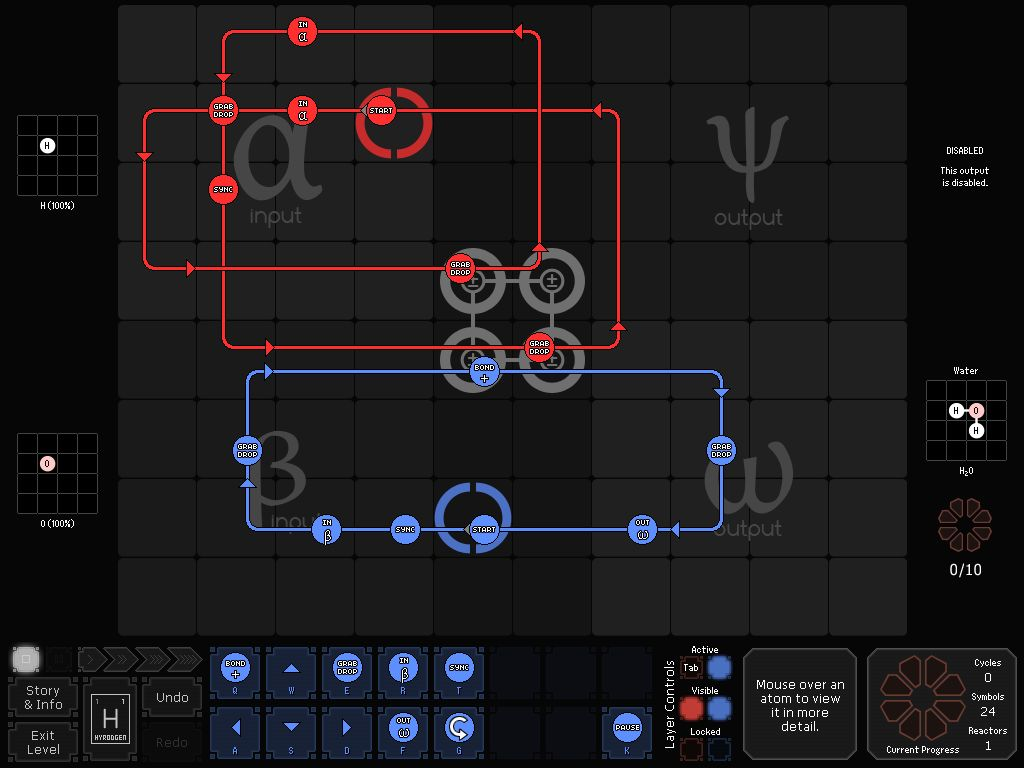
\includegraphics[width=350px,clip=true]{SpaceChem.jpg}
    \caption{SpaceChem}
    \label{fig:spaceChem}
\end{figure}

\begin{figure}[H]
    \centering
      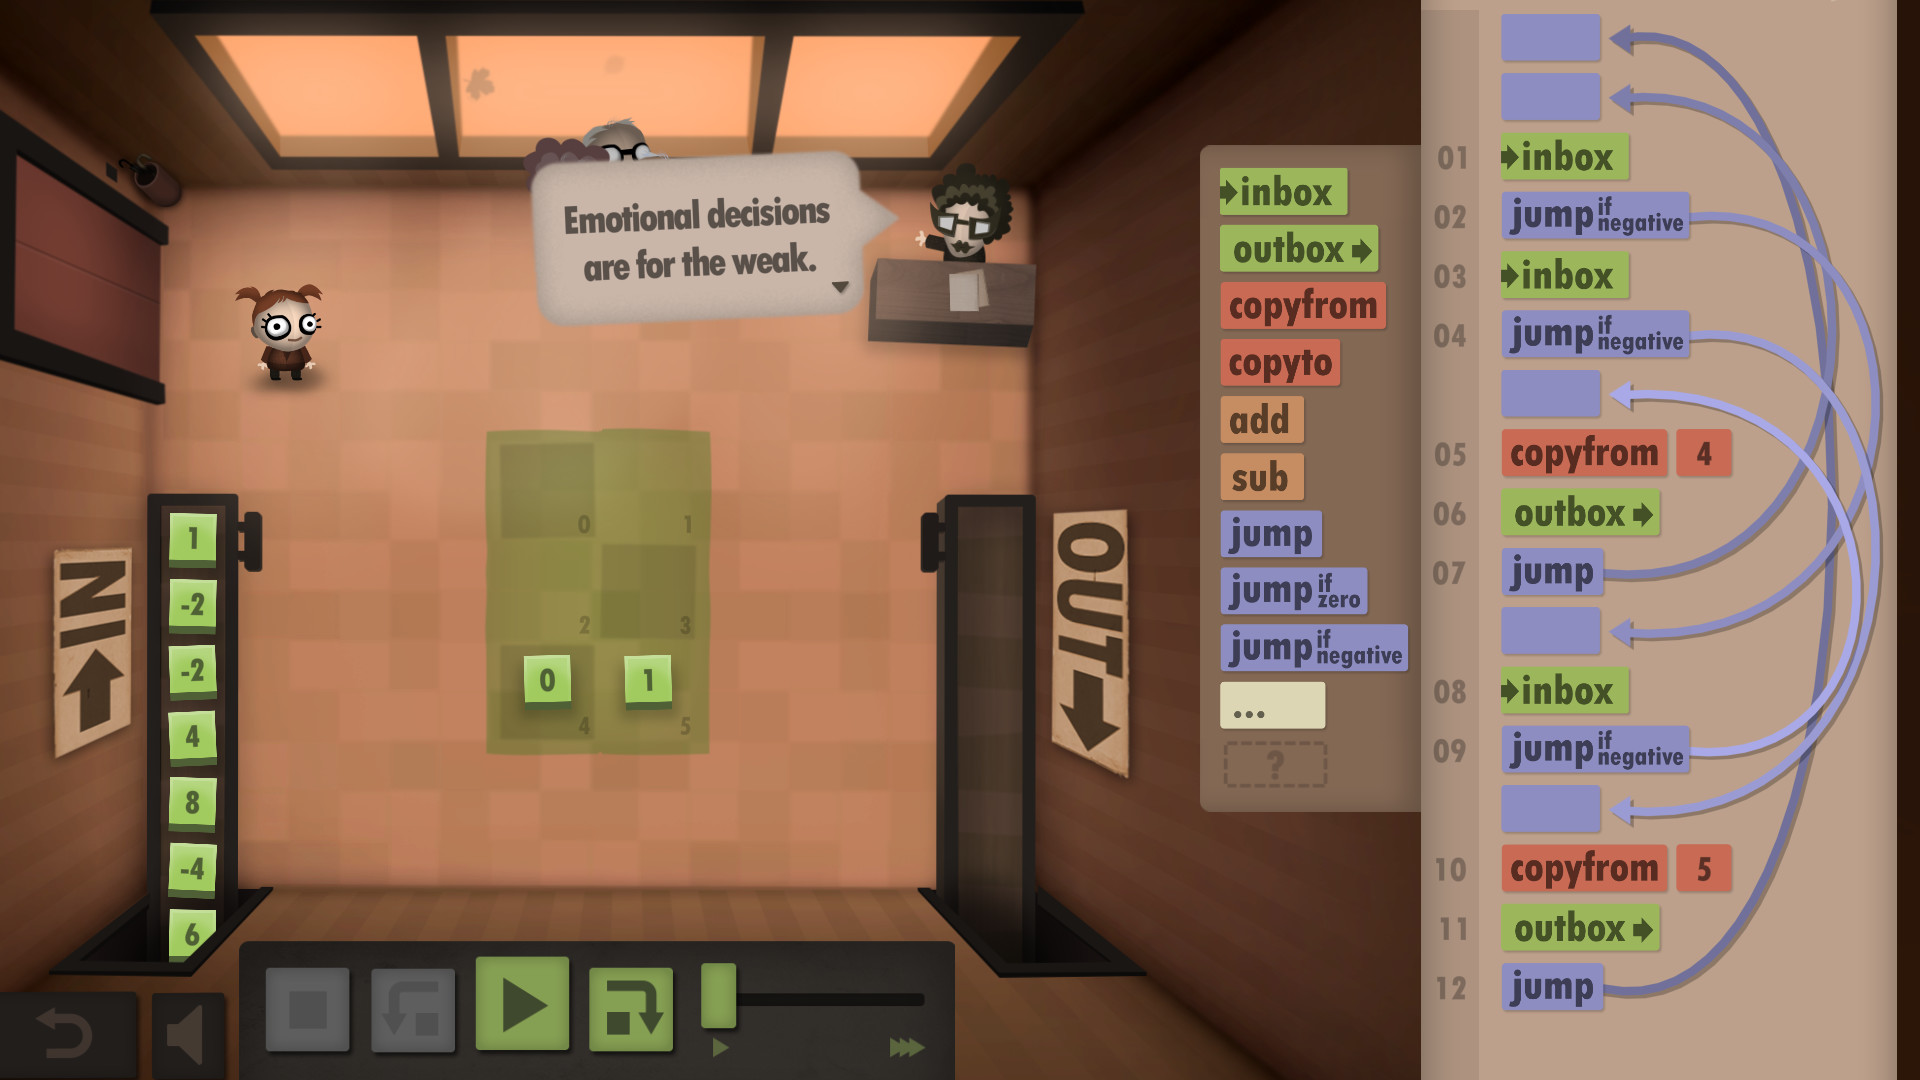
\includegraphics[width=350px,clip=true]{HRSM.jpg}
    \caption{Human Resource Machine}
    \label{fig:hsrm}
\end{figure}

\begin{figure}[H]
    \centering
      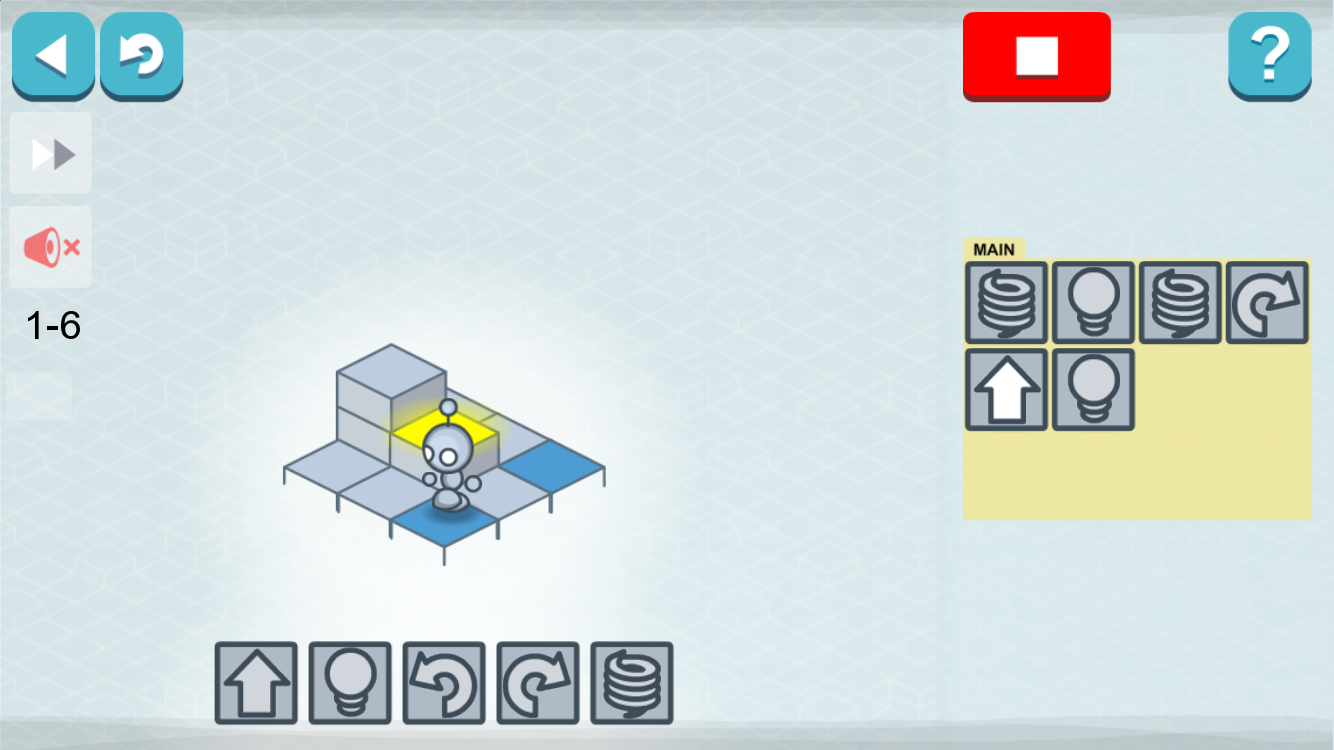
\includegraphics[width=350px,clip=true]{LightBot.png}
    \caption{LightBot}
    \label{fig:lightbot}
\end{figure}

Aunque si bien es cierto que los juegos que más se relacionan con el PC suelen ser juegos muy ligados a la algoritmia y la programación, no se puede decir que sean los únicos, los juegos de puzles al huso como Portal\cite{portal} o Portal 2\cite{portal2} (Figuras \ref{fig:portal} y \ref{fig:portal2}) también ayudan a entrenar aspectos del PC como la Generalización y el Análisis de datos.

\begin{figure}[H]
    \centering
      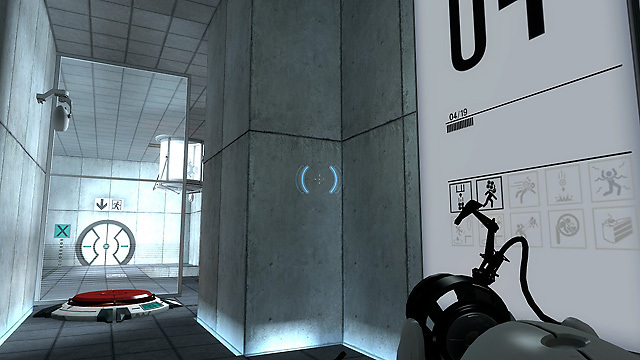
\includegraphics[width=350px,clip=true]{Portal.jpg}
    \caption{Portal}
    \label{fig:portal}
\end{figure}

\begin{figure}[H]
    \centering
      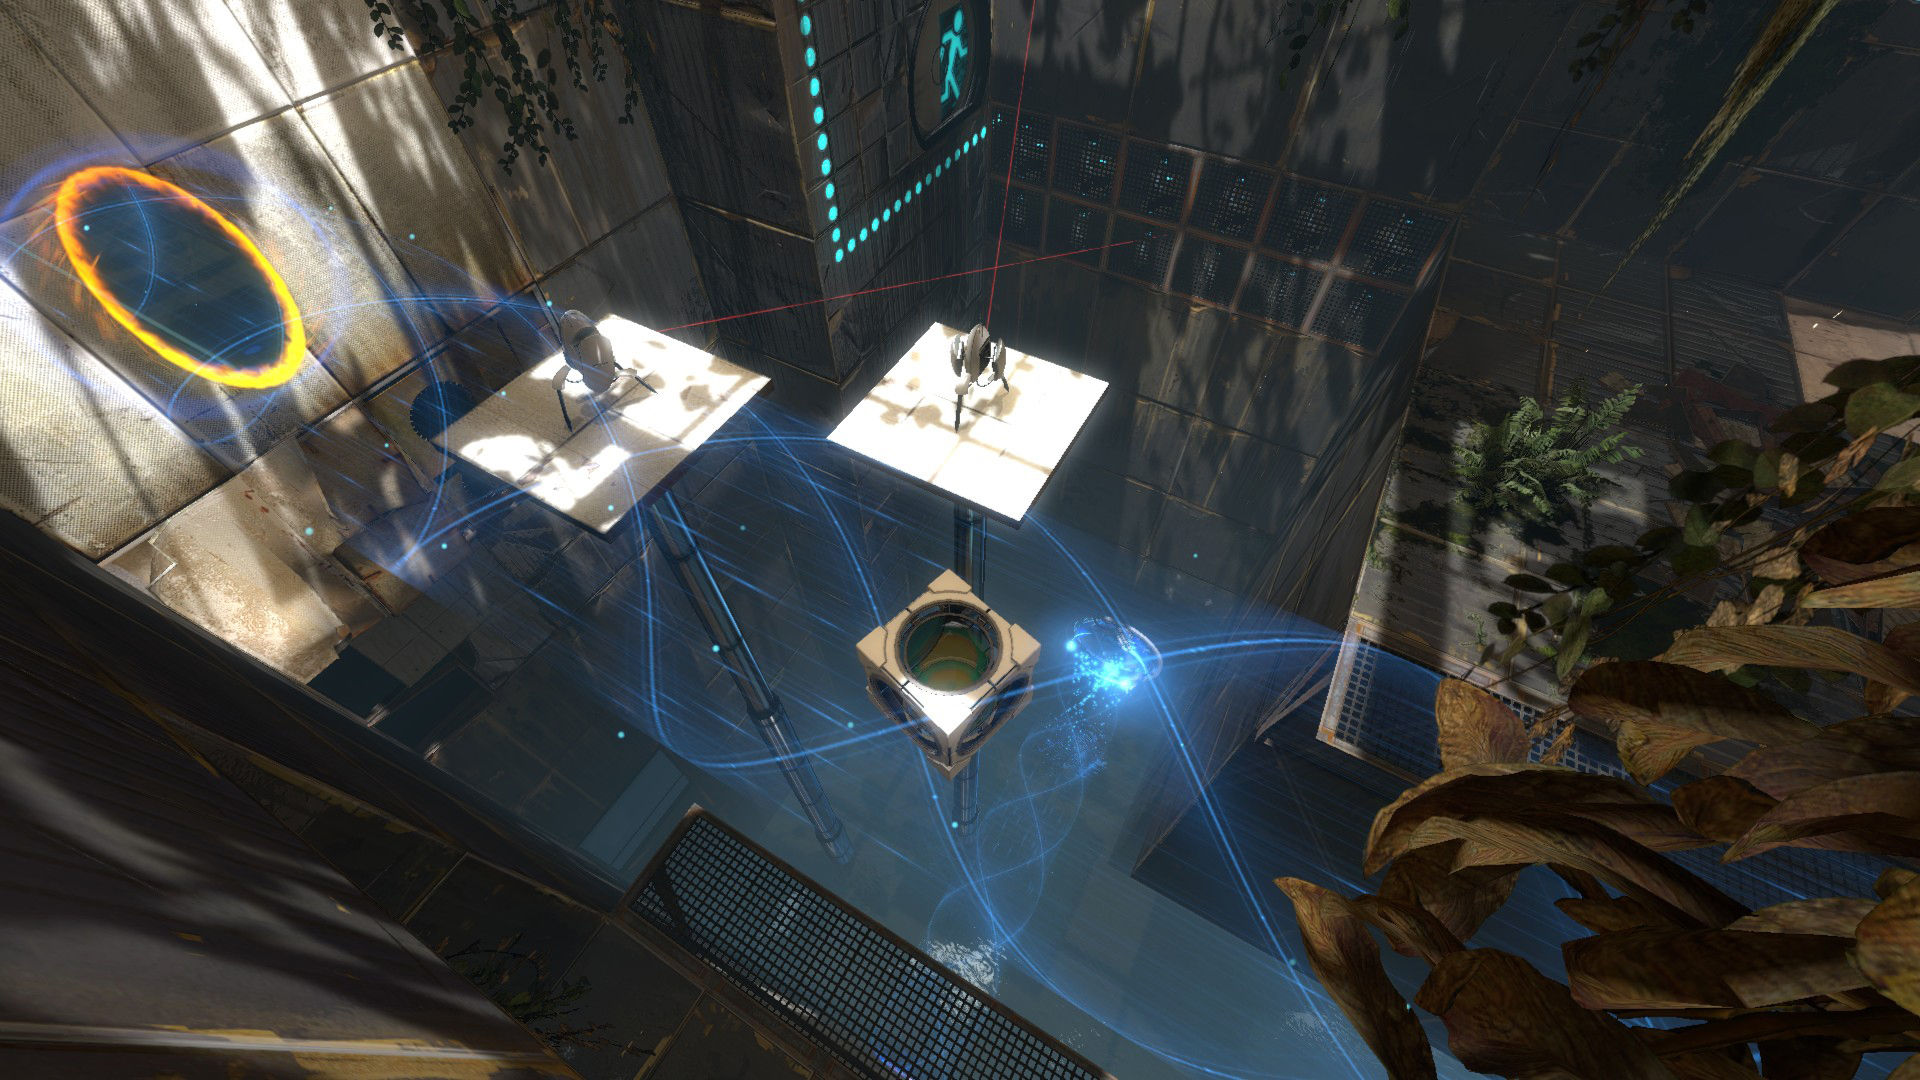
\includegraphics[width=350px,clip=true]{Portal 2.jpg}
    \caption{Portal 2}
    \label{fig:portal2}
\end{figure}

Por otra parte tenemos un ejemplo muy curioso como lo es Minecraft\cite{Minecraft}, que pese a ser un juego donde suele primar la creatividad, la 'Redstone' (Figura \ref{fig:minecraft}) (Una mecánica que simula la electricidad dentro del juego) permite la creación de puertas lógicas y mini CPUs virtuales dentro del propio juego. Esto claramente ayuda a la gente que interactúa con estas mecánicasa desarrollar su PC, de forma que se podría considerar a Minecraft como un juego apto para desarrollar el PC en niños y adolescentes.

\begin{figure}[H]
    \centering
      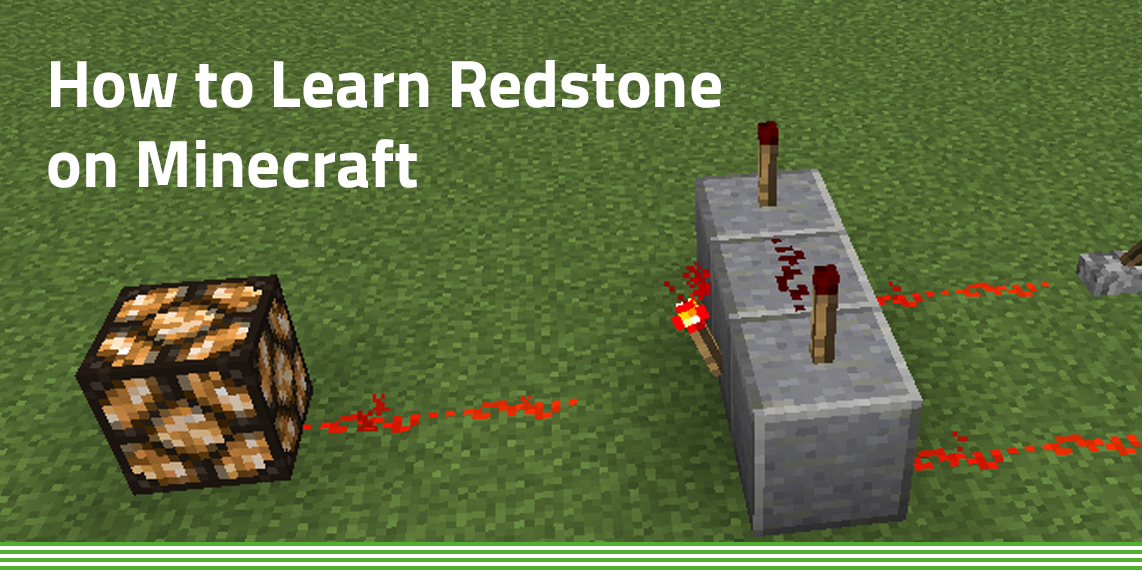
\includegraphics[width=350px,clip=true]{Minecraft.jpg}
    \caption{Minecraft}
    \label{fig:minecraft}
\end{figure}


Sin embargo, aunque sea verdad que Portal 1 o Minecraft son juegos que puedan ayudar al desarrollo del PC, eso no quita que la grandísima mayoría (si no todos) los juegos que hay actualmente como listados apoyo al PC tienden a estar centrados en cosas como la informática o la tecnología. El desarrollo de Ecorescue nace en parte por un desdeo de hacer un juego didácitco que sirva para el desarrollo del PC, pero que a su vez se aleje de el 'estereotipo' de videojuego sobre programar, de forma que de cara a presentar el proyecto en las aulas no se perciba como un ejercicio de informática en lugar de como un videojuego.